\section{Setup}
\frame{\tableofcontents[currentsection, hideothersubsections]}

\begin{frame}
\frametitle{Experiment Setup: Task}

\begin{figure}
    \centering
    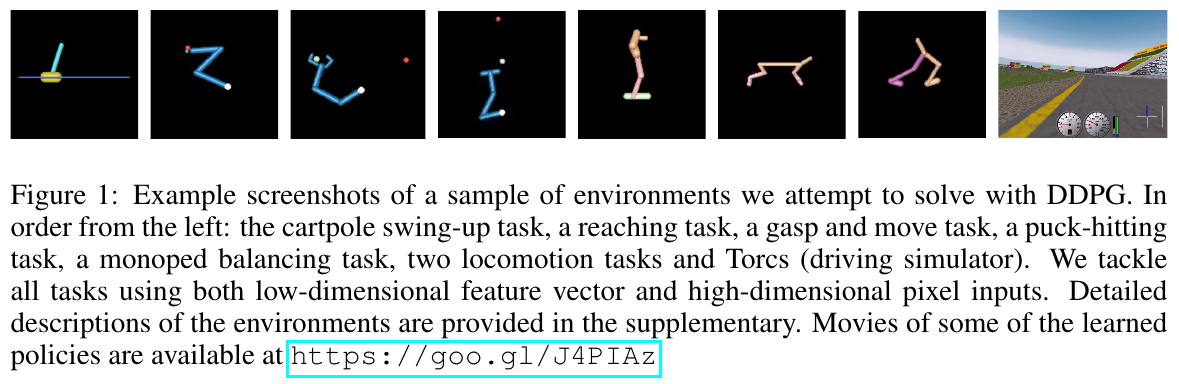
\includegraphics[scale=0.3]{fig_1}
\end{figure}

\begin{itemize}
  \item 20 simulated physics task,
  \begin{itemize}
    \item gripperRandom:
    Agent must use an arm with gripper appendage to grasp an object and manuver the object, which
    are initialized in random locations
    % \item reacher3daRandomTarget:
    % Agent is required to move a 7-DOF human-like arm from random starting locations to random target positions.
    \item reacherObstacle:
    Agent is required to move a 5-DOF arm around an obstacle to a randomized target position.
  \end{itemize}
  \item using both a low-dimensional state description (such as joint angles and positions) and high-dimensional renderings of the environment
\end{itemize}

\end{frame}

\begin{frame}
\frametitle{Experiment Setup: Task}

\begin{figure}
    \centering
    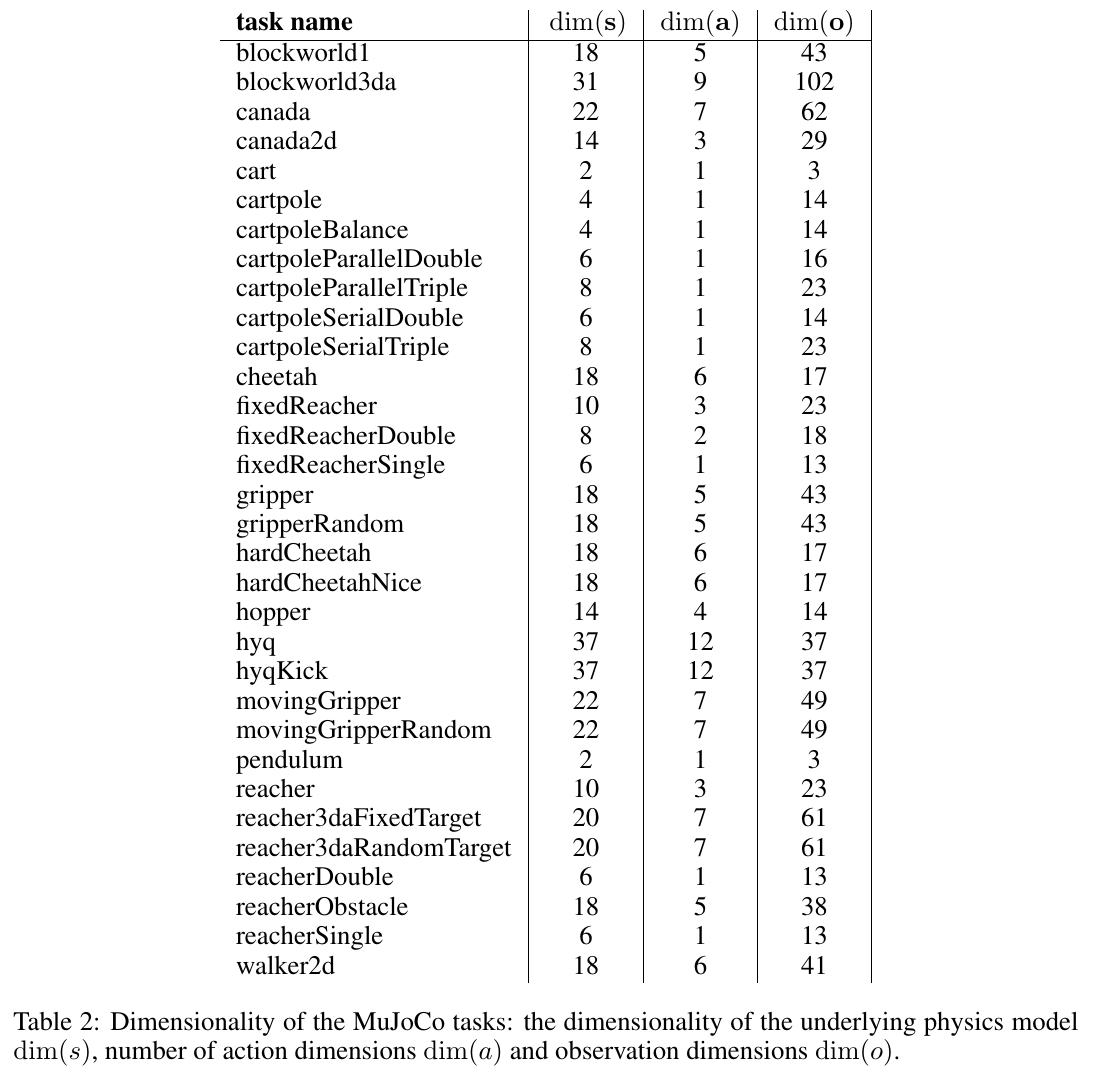
\includegraphics[scale=0.25]{task_dim}
\end{figure}

\end{frame}


\begin{frame}
\frametitle{Experiment Setup: Baseline, Assumptions}

Assumption:
\begin{itemize}
  \item env is MDP, the environment is fully-observed
\end{itemize}

Baseline:
\begin{itemize}
  \item the mean return from a naive policy which samples actions from
  a uniform distribution over the valid action space
  \item iLQG, a planning based solver with full access to
  the underlying physical model and its derivatives.
  \item normalize scores so that the naive policy has
  a mean score of 0 and iLQG has a mean score of 1.
\end{itemize}

\end{frame}

